\documentclass[a4paper,11pt]{article}

\usepackage[left= 1.5cm,text={18cm, 25cm},top=2.5cm]{geometry}
\usepackage[utf8]{inputenc}
\usepackage[T1]{fontenc}
\usepackage{times}
\usepackage{paralist}
\usepackage{graphicx}
\graphicspath{ {./img/} }
\usepackage{textcomp}
\usepackage{enumitem}
\usepackage{amssymb}
\usepackage{amsmath}
\usepackage{xcolor}
\usepackage[ddmmyyyy]{datetime}
\usepackage{array}
\pagestyle{plain}
\pagenumbering{arabic}
\usepackage[czech]{babel}
\usepackage{lmodern}
\usepackage{float}


\renewcommand*\contentsname{Obsah}

\newdateformat{mydate}{\twodigit{\THEDAY}.{ }\shortmonthname[\THEMONTH] \THEYEAR}

\pagenumbering{arabic}

\usepackage{url}
\DeclareUrlCommand\url{\def\UrlLeft{<}\def\UrlRight{>} \urlstyle{tt}}

% \usepackage{indentfirst}

\begin{document}
\selectlanguage{czech}

\begin{titlepage}
\begin{center}
    {\Huge \textsc{Vysoké učení technické v Brně}}
\vspace{\stretch{0.01}}
    
    {\LARGE \uppercase{FAKULTA INFORMAČNÍCH TECHNOLOGIÍ}}
    
\begin{figure}[h]
\vspace{5.0cm}
\centering

\includegraphics[scale=0.15]{logo.png}
\vspace{-10.0cm}
\end{figure}
    
\vspace{\stretch{0.382}}
	{\LARGE Projekt IMS, 2019Z}
\vspace{\stretch{0.02}}

	{\Huge \textbf{10 - Celulární automaty}}
\vspace{\stretch{0.02}}\\

{\LARGE {Hrabošová krize}}\\

\begin{figure}[h]
\centering
{\Large {\mydate\today}}
\vspace{6cm}
\end{figure}

\end{center}
\begin{compactitem}
\item[] \textbf{Autoři:}
\item[] Marek Petr, xmarek66
\item[] Vanický Jozef, xvanic09
\end{compactitem}

\end{titlepage}

\tableofcontents
\newpage

\section{Úvod}
Práce vznikla v rámci předmětu Modelování a simulace na Fakultě informačních technologií VUT v Brně. Popisuje model (\cite{slajdy}, snímek č. 7) celulárního automatu (\cite{slajdy} č. 209), jehož úkolem je predikce intenzity populace hraboše polního \textit{(Microtus arvalis)} a jeho regulace. Cílem práce je porovnání výsledků experimentů - jednotlivých protiopatření vůči hraboši polnímu na modelu popsaném ve článku \cite{OurCA}. Jde o protiopatření hloubkové orby, plytké orby a použití chemické látky - Stutox II s účinnou látkou Fosfidem zinečnatým. Tato protiopatření jsou dále popsaná ve článcích \verb|\cite{}|\verb|\cite{}|. 

Experimenty slouží k demonstraci účinnosti jednotlivých protiopatření na populaci hraboše polního. Předmětem zkoumání je grafický výstup zobrazující nárůst  a  pokles hustoty populace hraboše v jednotlivých měsících na poli o velikosti 1 hektaru. 

\subsection{Zdroje faktů}
Jako zdroje informací byly použity odborné publikace\cite{prubehvyvoje} a další zdroje dat\cite{letak}, které se zabývají problematikou přemnožení tohoto hlodavce a také vědecké články zabývající se tvorbou celulárního automatu na tuto problematiku \cite{OurCA}. Důvěryhodnost informací byla ověřována vyhledáváním těchto informací v jiných odborných publikacích \cite{fluktuace} \cite{prubehvyvoje} a potvrzená odborníky z praxe, doktorem Emilem Tkadlecem z ústavu bilogie obratlovců Akademie věd ČR, který se zabývá populační dynamikou živočišních populací a jejich modelováním a Agronomem Gabrielem Konczem ze Zemědělského družstva v Períně SK.

\subsection{Ověření validity/funkčnosti}
Ověřování validity modelu bylo vykonáváno průběžnou simulací modelu, jež odpovídala chování populace hraboše polního popisovaného publikacemi \cite{letak}\cite{fluktuace}\cite{prubehvyvoje}\cite{Voles-popul-data:online}\cite{diplom-Tkadlec}. Úbytek populace v zimním období a populační exploze projevující se od jarních měsíců odpovídá také naměřeným údajům \cite{Winter-temp:online}. Experimenty byly ověřovány na základě odborných článků, které popisují přibližně stejnou účinnost jednotlivých protiopatření a konzultací s odborníkem z Agroprůmyslu - Gabrielem Konczem ze Zemědělského družstva se sídlem v Períně na Slovensku.   

\section{Rozbor tématu, použitých metod a technologií TODO}
Abychom byli schopni vytvořit model populační exploze, je nutné znát údaje o hraboši polním \textit{(Microtus arvalis)} a jeho chování v průběhu roku.
 Zároveň je nutné znát vliv zimního období na hraboše polního. Rozmnožovací období trvá 7 měsíců a nastává od třetího do desátého měsíce.\cite{diplom-Tkadlec} Vlivem nízké teploty a nedostatku potravy v zimě populace hraboše klesá. Koncem zimy je populace hraboše nejmenší, naopak nejvíce jedinců pozorujeme na konci léta.\cite{Winter-temp:online} Březost samice je 19 až 21 dní. Jedna samice za rok vrhne průměrně 5 až 6 mláďat\cite{diplom-Tkadlec}, z čehož jsme vypočítali reprodukční koeficient pro model.\cite{OurCA}. Na jednom hektaru se vyskytuje maximálně 3000 až 7000 jedinců. \verb|\cite{}|

\subsection{Popis použitých postupů}
Při práci byl využit objektově orientovaný jazyk C++. Tento jazyk je díky své rychlosti vhodný pro vytváření simulací, které mohou být výpočetně náročné a jazyk s nižší rychlostí výpočtu by mohl simulaci výrazně zpomalit. 

K vizualizaci jednotlivých stavů celulárního automatu byla použita grafická knihovna OpenCV2 \cite{opencv2}, ve které lze snadno implementovat vytváření jednoduchých obrázků. 

\subsection{Popis použitých metod a technologií}
Pro účely implementace celulárního automatu byl použit jazyk C++ a jeho standardní knihovny. Grafické zobrazení výsledků zajišťuje knihovna OpenCV.

\section{Koncepce modelu}
Koncepce modelu vychází z informací popsaných v předchozí kapitole. Každá buňka obsahuje hodnotu, která udává populaci v dané buňce. Model pro výpočet hustoty populace byl převzat z vědecké článku \cite{OurCA} časopisu Ecological Modelling vydavatelství Elsevier Ltd. Populace je v něm modelována následujícími rovnicemi:
\begin{equation}
N_{x,y}(t+1) = H(N_{x,y}(t) + \alpha*N_{x,y}(t) + \beta*N_{x,y}(t)^2 + \gamma\delta^2*N_{x,y}(t))
\end{equation}
\begin{equation}
\delta^2*N_{x,y} = N_{x,y-1} + N_{x,y+1} + N_{x+1,y} + N_{x-1,y} - 4N_{x,y}
\end{equation}
\( N_{x,y}(t) \) - stav buňky na souřadnicích x,y v čase t\ \\
\( \delta^2*N_{x,y} \) - diskretizovaný difuzní operátor kontrolující šíření buněk \\
\( \alpha \) - porodnost \\
\( \beta \) - úmrtnost \\
\( \gamma \) - migrační operátor\\


\section{Architektura simulačního modelu}
Simulátor je složen ze dvou tříd \emph{Cell},\emph{Grid} a \emph{Image}. Mřížka celulárního automatu má rozměry 100x100 a představuje jeden hektár. Počáteční stav automatu je generován náhodně. Simulace vždy běží po dobu 48 měsíců.

\subsection{Třída Cell}
Třída \emph{Cell} implementuje jednu buňku celulárního automatu. Obsahuje informace o stavu této buňky, tedy její souřadnice a hustotu. Buňka odpovídá 1x1m pole.

\subsection{Třída Grid}
Třída grid reprezentuje mřížku celulárního automatu a zodpovídá za jeho chování. Také obsahuje základní informace modelu. Například velikost mřížky, porodnost, úmrtnost a další. Dále se v ní nachází metody umožňující spuštění a řízení simulace. V této třídě se také nachází metoda emph{init\_present\_grid()}. Ta vytváří čtyřicet shluků maximálně dvaceti buněk, které náhodně rozmístí do mřížky.
Ovšem nejdůležitější metodou je \emph{get\_future\_grid()}, která ze současného stavu automatu vypočítá ten následující. V ní je definováno chování modelu i jeho změna při vykonávání jednotlivých experimentů.

\subsection{Třída Image}
Tato třída zajišťuje zobrazení grafického výsledku jednotlivých běhů simulace. Její hlavní metodou je \emph{create\_image()}, která vykresluje současný stav mřížky automatu.


\section{Podstata simulačních experimentů a jejich průbeh}
Cílem experimentů je demonstrovat šíření populace hraboše polního v úseku 1 hektar a jeho regulaci za použití jednotlivých protiopatření. Předmětem zkoumání je grafický výstup zobrazující nárůst a pokles populace a její migraci. 
\subsection{Postup experimentování}
Byly vykonány čtyři experimenty, jejichž výsledky byly konzultovány s Agronomem Gabrielem Konczem ze Zemědělského družstva v Períně na Slovensku. Výsledky byly ověřeny za použití zdrojů a dát\cite{Voles-popul-data:online}
\subsection{Dokumentace jednotlivých experimentů}
Experimenty byly vykonané v matici 100x100, která reprezentuje 1 hektar orné půdy. Jedna buňka reprezentuje populaci hrabošů na 1$m^{2}$. Simulace každého experimentu začíná ve třetím měsíci, kdy populace začíná růst. Všechny experimenty měly stejný reprodukční koeficient spočítaný na základě parametru porodnosti, úmrtnosti a migrace. Protiopatření je v experimentech použito jednou za rok, přičemž experimenty byly vykonávány po dobu 4 let.

\subsubsection{Experiment 1}
\begin{figure}[h]
\begin{center}  
    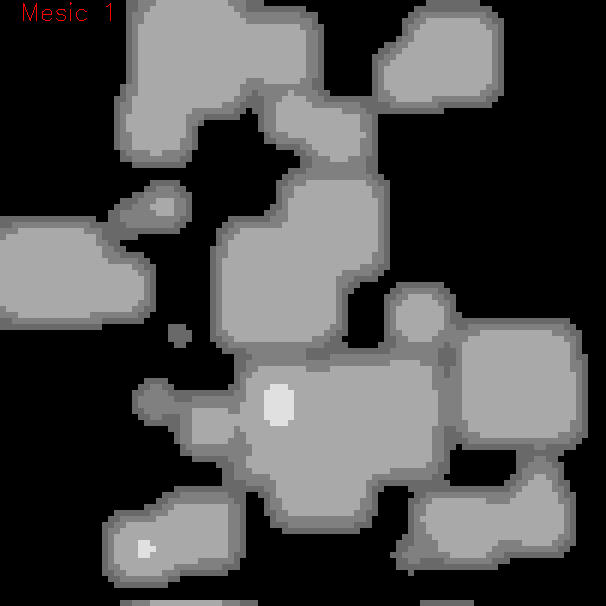
\includegraphics[width=.4\linewidth]{bez_regul1.png}
    \caption{Stav populace v lednu}
    \label{pic:exp1_obr1}
\end{center}
\end{figure}

V tomto experimentu nebylo použito žádné protiopatření. Cílem experimentu bylo validovat model, predikovat nárůst populace v průběhu letních období začínajících od března a naopak pokles populace v měsících zimních, tedy listopad až únor. 

\begin{figure}[h]
\begin{center}
    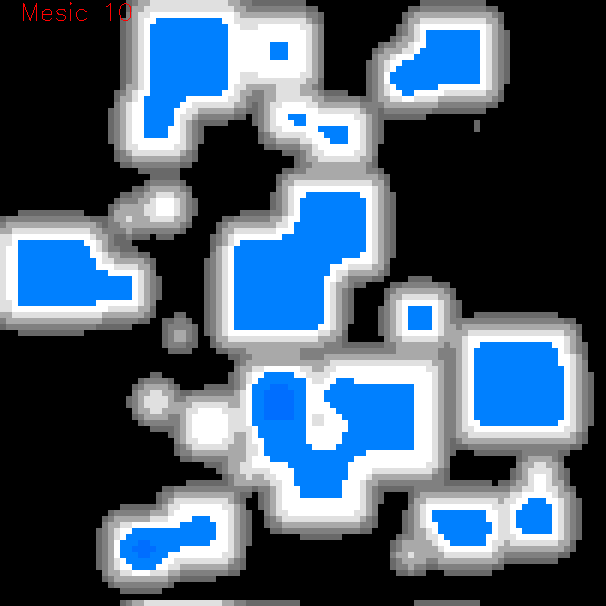
\includegraphics[width=.4\linewidth]{bez_regul10.png}
    \caption{Stav populace v říjnu}
    \label{pic:exp1_obr2}
\end{center}
\end{figure}

Výsledek experimentu prokázal validitu modelu vůči informací z výzkumů \cite{fluktuace} a datům \cite{Voles-popul-data:online}
\subsubsection{Experiment 2}
\textbf{OBRAZOK PRED ORBOU}
V experimentě byly použity protiopatření hluboké orby, která by podle Marty Heroldové z Ústavu ekologie lesa Lesnícké a dřevářské fakulty MENDELU měla zredukovat populaci přibližně o 50\%, přičemž je vykonávána jednou ročně v říjnu. 

V experimentě byly použity protiopatření hluboké orby, která by podle Marty Heroldové z Ústavu ekologie lesa Lesnícké a dřevářské fakulty MENDELU měla zredukovat populaci přibližně o 50\%, přičemž je vykonávána jednou ročně v říjnu. 

\begin{figure}[h]
\begin{center}
    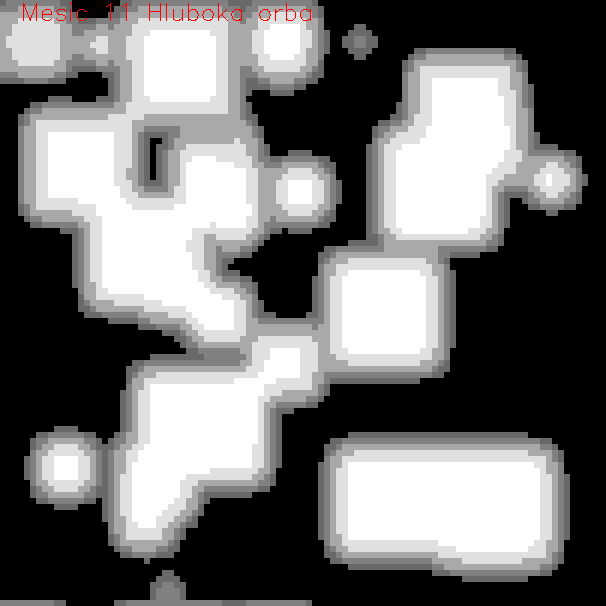
\includegraphics[width=.4\linewidth]{hlub_orba11.png}
    \caption{Stav populace po hluboké orbě}
    \label{exp2_obr2}
\end{center}
\end{figure}

Výsledek experimentu prokázal přibližně poloviční pokles populace. Jelikož se hluboká orba vykonává před zimou, je efektivním způsobem, jak redukovat stav hrabošů na několik měsíců dopředu, což prokazuje tento experiment.
\newpage

\subsubsection{Experiment 3}
\textbf{OBRAZOK PRED ORBOU}
V experimentu byly použity protiopatření mělké orby, která podle dostupných informací od Agronoma Gabriela Koncza redukuje populaci přibližně o 20\%, přičemž je vykonávána jednou ročně v dubnu. 

\begin{figure}[h]
\begin{center}
    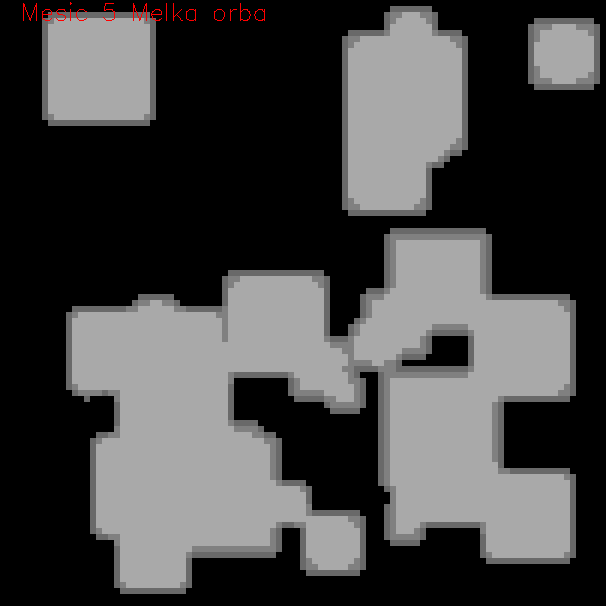
\includegraphics[width=.4\linewidth]{melka_orba5.png}
    \caption{Stav populace před mělkou orbou}
    \label{exp3_obr2}
\end{center}
\end{figure}

Výsledek experimentu prokázal mírný pokles populace. Mělká orba vykonávána na jaře zasahuje až 15 cm pod povrch a jejím cílem je provzdušnit půdu. Snížení počtu hrabošů dosahuje do 20\% a to kvůli nízkému zásahu pod povrch země, čímž jsou zasaženy jenom plytké nory. 

\newpage
\subsubsection{Experiment 4}
Tento experiment testuje dopad jedu Stutox II použitého v květnu každý rok na rostoucí populaci.

\begin{figure}[h]
\begin{center}
    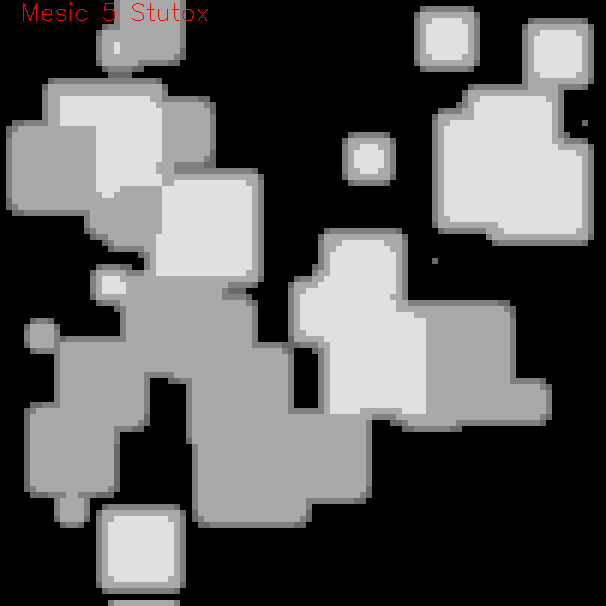
\includegraphics[width=.4\linewidth]{stutox5.png}
    \caption{Stav populace před použitím jedu Stutox II}
    \label{exp4_obr1}
\end{center}
\end{figure}

Výsledek prokázal významný dopad na počty hrabošů, ale k okamžité decimaci populace nedošlo. Nicméně velké snížení populace se přeneslo do zimy, kde populace téměř úplně vymřela. Další rok se populace ve velmi malém rozsahu pokusila o obnovení, ale její počty nebyly k tomuto účelu dostatečné a přes zimu se zhroutila úplně.

\begin{figure}[h]
\begin{center}
    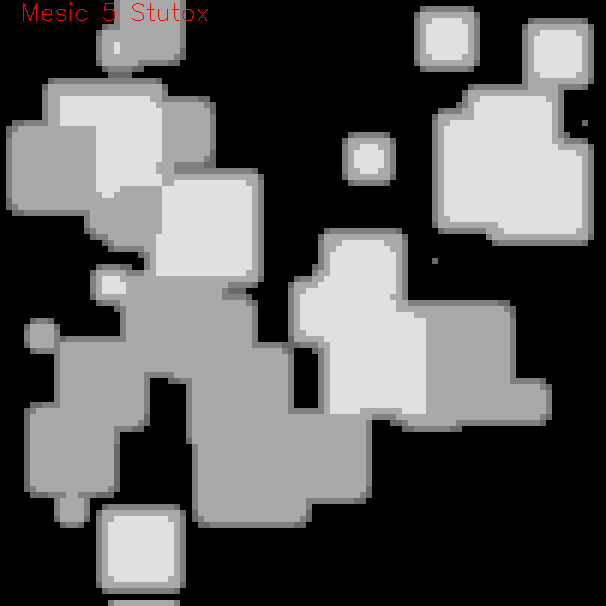
\includegraphics[width=.4\linewidth]{stutox5.png}
    \caption{Stav populace před použitím jedu Stutox II}
    \label{exp4_obr2}
\end{center}
\end{figure}

\newpage
\subsection{Zhodnocení experimentů}


\section{Závěr}


\section{Literatura}


\newpage
\bibliographystyle{czplain}
\renewcommand{\refname}{\section{Literatura}}
\bibliography{dokumentace}
\end{document}